%%
%% 研究報告用スイッチ
%% [techrep]
%%
%% 欧文表記無しのスイッチ(etitle,jkeyword,eabstract,ekeywordは任意)
%% [noauthor]
%%

%\documentclass[submit,techreq]{ipsj}
\documentclass[submit,techreq,noauthor]{ipsj}


\usepackage[dvips]{graphicx}
\usepackage{latexsym}

\def\Underline{\setbox0\hbox\bgroup\let\\\endUnderline}
\def\endUnderline{\vphantom{y}\egroup\smash{\underline{\box0}}\\}
\def\|{\verb|}


\begin{document}

% Title %%%%%%%%%%%%%%%%%%%%%%%%%%%%%%%%%
\title{強い型によるOSの開発手法の提案}

\affiliate{METASEPI}{Metasepi Project}
\affiliate{OCAML-NAGOYA}{ocaml-nagoya}

\author{岡部 究}{Kiwamu Okabe}{METASEPI}[kiwamu@debian.or.jp]
\author{水野 洋樹}{Hiroki MIZUNO}{OCAML-NAGOYA}[mzp@ocaml.jp]
\author{瀬川 秀一}{Hidekazu SEGAWA}{}[]

\begin{abstract}
現在でもOSはC言語によって設計されている.
一方アプリケーションは強い型付けの言語を用いた安全な設計手法が確立されている.
本稿ではその設計手法をOSにも適用する手法を提案する.
\end{abstract}

\begin{jkeyword}
プログラミング・シンポジウム,プログラミング言語,コンパイラ,Haskell,OS
\end{jkeyword}

\maketitle

% Body %%%%%%%%%%%%%%%%%%%%%%%%%%%%%%%%%
\section{はじめに}

筆者らはAjhc Haskellコンパイラ\cite{ajhc}を開発している.
Ajhcは実用化可能なOSを設計可能な型推論をそなえたコンパイラを目指している.
本稿ではAjhcを使ったOSの開発手法を提案し,その手法を小規模ソフトウェアに対して適用/評価する.
最後に今後の研究計画について述べる.

\section{OS開発における既存手法の問題}
\label{sec:problems}

ソフトウェア開発について実行時エラーの削減は重要なテーマである.
エラー削減には設計後のテストや検証など多くの手法があり,
その一つとして設計時に強い型付けの言語を用いる手法も提案されている.
一方LinuxやBSDのような実用化されたOSの開発において
主に使われているプログラミング言語はC言語である.
C言語はMLやHaskellのような型推論をそなえた言語より弱い型付けであるために
しばしば実行時エラーを引き起こす.
アプリケーション領域ではこのC言語は積極的に使われることはなく,
より強い型付けの言語が実用化設計に応用されている.
研究レベルにおいて,
型推論をそなえた強い型付け言語でOSを設計する試みは複数存在する
\cite{funk}\cite{snowflake-os}\cite{house}.
しかしこれらのOSはLinuxやBSDのようにデスクトップ/サーバ用途として実用化されていない.
筆者らは上記のOSが実用化されていない原因は主に3つに大別できると考える.

一つ目は,実用化に辿り着くまでプロジェクト参加者の気力が継続できないということである.
実用化されたLinuxのようなOSはLinux kernelの動作するデスクトップでLinux kernel自体を開発している.
彼等はまた開発以外の日常のデスクトップ用途にもLinux kernelを使用する.
このような開発スタイルはドッグフードと属に呼ばれている.
この開発サイクルで自然に実用的なテストが行なわれ,OSの品質は向上する.
OS開発ではこのドッグフード開発にすばやく辿り着く手法を採用する必要がある.

二つ目は,ハードウェア割込をポーリングで検出していることである.
型推論を持つ言語実装の多くは再入可能ではない.
そのためハードウェア割込は言語のランタイムで受け取り,
OS実装側は定期的にランタイムにためられたイベント通知をラ引き上げる必要がある.
実用化されたOSのほとんどは割込をイベントドリブンでOS実装が直接引き上げる.
つまりUNIX誕生から長年つちかわれたOS設計のノウハウを捨てて,
まったく新しい設計検討をドッグフード開発を開始するまで継続しなければならない.

最後に,これらのOSはC言語で設計された既存のデバイスドライバと共存することができない.
OSの存在意義はアプリケーションを動作させるためであるが,
そのためにはコンピュータに接続されたデバイスを抽象化してアプリケーション側に見せてやる必要がある.
世界中には膨大な種類のデバイスが存在し,それぞれに異なるドライバ実装が必要である.
これらのOSではドッグフード開発に必要なドライバ群をすべてゼロから再実装する必要がある.

\section{本稿で提案する開発手法}

筆者らは上記の問題を解決するために\textbf{スナッチ設計}という手法を提案する.
スナッチ設計ではOSをゼロから設計することはせず,既存のC言語によって設計されたOSのソースコードを元に少しずつC言語による設計に強い型を付ける.
この手法によってドッグフード開発をしながら強い型を持つ言語によるOS開発が可能で,
さらに既存のデバイスドライバを再利用することもできる.

既存の再入可能でないコンパイラでは,
イベントドリブンで設計されたOSをスナッチ設計することができない.
そこでスナッチ設計を行なうためのコンパイラを作成する基礎となるコンパイラを選定するために
``hoge''と印字するだけのプログラムをコンパイルして比較評価した
(\tabref{tab:compilerlist}).
各評価値が小さいほどPOSIX依存度が低いことを示している.
評価対象の実装の中ではjhc\cite{jhc}がずば抜けて良い特性を持っていることがわかる.
しかしjhcは再入可能なバイナリを扱えず,もちろんスレッドさえサポートされていない.
そこで筆者らはjhcをスレッドと再入可能をサポートしたAjhcコンパイラを開発した\cite{j-ikamusume5}.

\begin{table}[tb]
\caption{``hoge''と印字するプログラムに見るコンパイラの特性}
\label{tab:compilerlist}
\hbox to\hsize{\hfil
\begin{tabular}{l|rrr}\hline\hline
コンパイラ実装	& サイズ & 未定義シンボル & 依存ライブラリ \\\hline
GHC-7.4.1	& 797228 B & 144 個 & 9 個 \\
SML\#-1.2.0	& 813460 B & 134 個 & 7 個 \\
OCaml-4.00.1	& 183348 B & 84  個 & 5 個 \\
MLton-20100608	& 170061 B & 71  個 & 5 個 \\
jhc-0.8.0	& 21248 B  & 20  個 & 3 個 \\\hline
\end{tabular}\hfil}
\end{table}

\section{開発手法の評価と考察}

スナッチ設計とAjhcの組合せをLinuxやBSDのような実用的なOSの開発に投入する前に
手法の評価を行なった.

最初に,RAMサイズが40kBのマイコン上でOSを搭載せずに直接Haskellコードを動作させた
\footnote{https://github.com/ajhc/demo-cortex-m3/tree/master/stm32f3-discovery}.
この評価では通常コンテキストとハードウェア割込コンテキストの両方をHaskell言語で実装した.
コンテキスト間の通信はポインタを経由するがAjhcの再入可能拡張が正常に動作することを実証した.
またjhcの小さなバイナリを生成する特性がOSの省メモリ化に寄与することも実証できた.

次に,スレッドをサポートした組込み向けOSの上に小さなTCP/IPプロトコルスタック
\footnote{https://savannah.nongnu.org/projects/lwip/}
を搭載し,その上で動作するネットワークアプリケーションをHaskellで作成した
\footnote{https://github.com/ajhc/demo-cortex-m3/tree/master/mbed-nxp-lpc1768}.
OSとプロトコルスタックのC言語実装とHaskell実装が協調動作させることが可能で,
まだHaskell化が進んでいない段階でもドッグフード開発に移行できることを実証できた.

\begin{figure}[h]
\centering
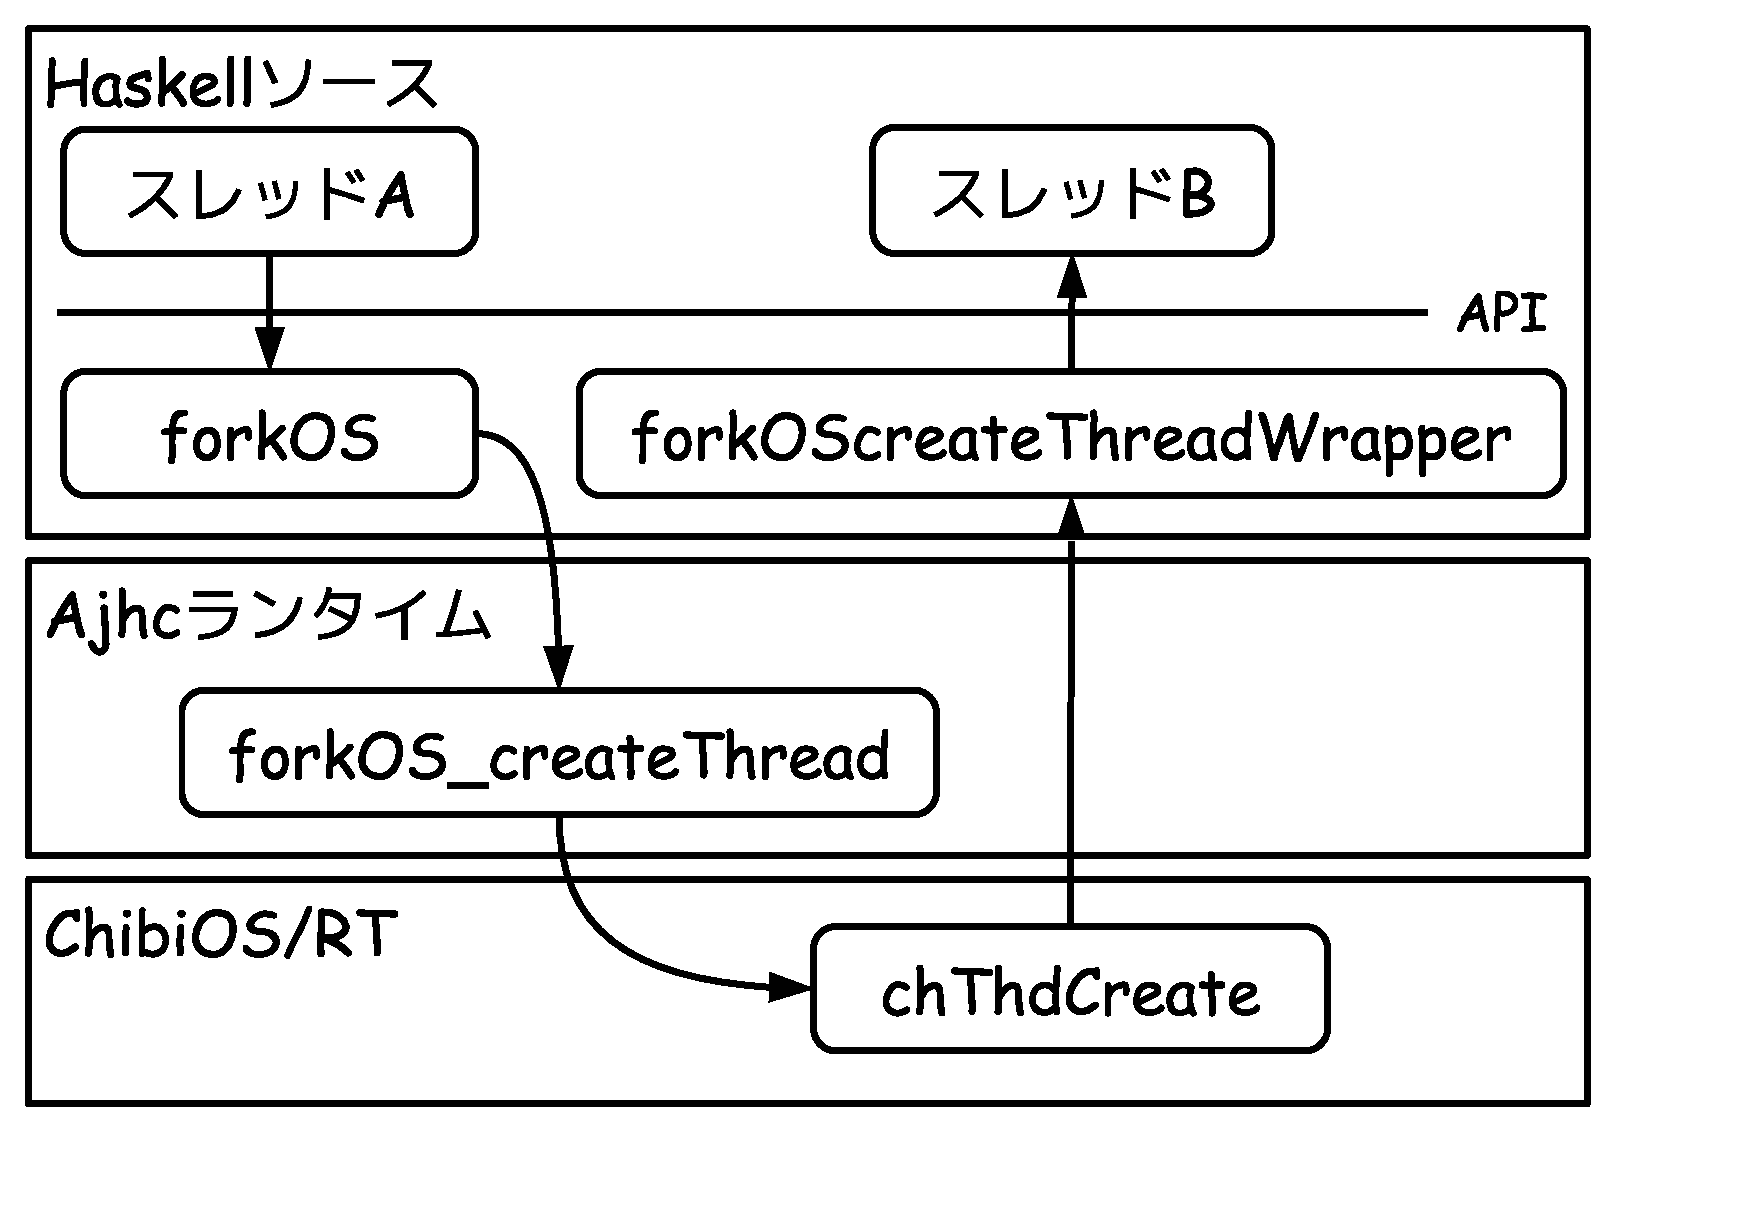
\includegraphics[width=75mm]{draw/chibi_thr.eps}
\caption{RTOSのスレッドを利用したHaskellスレッド実装}
\label{fig:forkos}
\end{figure}

最後に,組込み向けOS
\footnote{ChibiOS/RT http://www.chibios.org/}
のスレッドを使ってHaskell言語のスレッド(forkOS)を実装した
\footnote{https://github.com/metasepi/chibios-arafura}.
AjhcのHaskellスレッド実装を,
ランタイム側に用意されているforkOS\_createThread APIを独自ものに差し換えれば
POSIXスレッド以外のOS側スレッド実装を使って実現できるように変更した(図\ref{fig:forkos}).
Ajhcが再入可能であるだけではなくスレッドセーフであることを実証した.

\section{結論と今後の課題}

スナッチ設計とAjhcの組合せによって\ref{sec:problems}章
でのOS実用化の3つの障壁を解決する見込みがたった.
しかしその過程でいくつかの問題が見つかった.
一つ目,C言語の構造体のように構造の一部を局所的に更新する簡単な方法がないことがある.
これはGHCで使われているvector\footnote{http://hackage.haskell.org/package/vector}
ライブラリをAjhcに移植することで解決できると考えられる.
二つ目,コンテキスト間の状態共有方法がポインタのみでしか許されず,型を使った状態共有ができない.
これはMVar\footnote{http://hackage.haskell.org/package/base/docs/Control-Concurrent-MVar.html}
をAjhcで使用可能にすべきである.

今後は上記2つの問題を解決した後,
スナッチ設計によってNetBSD kernelの一部のデバイスドライバをHaskell化する予定である.
またjhc以外のスナッチ可能なコンパイラとして有望に思われるATS言語
\footnote{http://www.ats-lang.org/}
の調査を行なう.

\begin{acknowledgment}
偉大なHaskellコンパイラを産み出し,
誰もが望みを捨ててしまっていたOS領域にかすかな光をもたらしたJohn Meachamに感謝する.
\end{acknowledgment}

% BibTeX %%%%%%%%%%%%%%%%%%%%%%%%%%%%%%%%%
\bibliographystyle{ipsjunsrt}
\bibliography{../bibtex/reference,../bibtex/jreference}

\end{document}
